\documentclass[a4paper,10pt]{article}
\usepackage[polish]{babel}
\usepackage[utf8]{inputenc}
\usepackage{polski}
\usepackage[T1]{fontenc}
\frenchspacing
\usepackage{indentfirst}
\usepackage{graphicx}
%opening
\title{Projekt z przedmiotu Techniki Internetu}
\author{Konrad Maciałek}

\begin{document}

\maketitle
\newpage

\section{Cel projektu}
Zaprojektowanie i wykonanie aplikacji internetowej spełniającej poniższe warunki:
\begin{enumerate}
 \item Dowolna tematyka projektu
 \item Serwis dostępny przez przeglądarkę internetową
 \item Końcową warstwę prezentacji muszą stanowić poprawne składniowo i semantycznie dokumenty HTML
 \item Baza danych musi składać się z co najmniej trzech tabel, pomiędzy którymi istnieją relacje
 \item Serwis musi umożliwiać wprowadzanie danych do bazy, modyfikację i usuwanie danych poprzez przeglądarkę internetową (interfejs HTML)
 \item Musi istnieć część administracyjna serwisu (np. przeznaczona do uzupełniania danych w bazie) zabezpieczona (poprzez mechanizm logowania) przed nieautoryzowanym dostępem;
\end{enumerate}

\section{Założenia projektowe}
\subsection{Tematyka projektu}
Zaprojektowanie prostego serwisu sklepu sportowego, posiadającego kilka kategorii towarów. 
\paragraph{}
Serwis powinien umożliwiać:
\begin{enumerate}
 \item Przeglądanie listy oferowanych towarów.
 \item Dodawanie i usuwanie towarów z koszyka zakupów.
 \item Składanie zamówienia wraz z podaniem adresu wysyłki.
 \item Dodawanie, usuwanie i modyfikację towarów poprzez zabezpieczoną logowaniem sekcję administracyjną.
\end{enumerate}

\subsection{Wybór technologii}
Przyjęto poniższe założenia:
\subsubsection{Środowisko developerskie}
\begin{enumerate}
 \item System operacyjny: Linux
 \item Baza danych: SQLite
\end{enumerate}

\subsubsection{Środowisko produkcyjne}
\begin{enumerate}
 \item System operacyjny: Windows 
 \item Baza danych: Azure SQL Server
\end{enumerate}

\subsubsection{Hosting}
Microsoft Azure App Service
\subsubsection{Wybór technologii}
Z uwagi na założoną wieloplatformowość, do realizacji projektu wybrano technologię ASP.NET Core MVC w wersji 2.1.

\section{Wykonanie}
\subsection{Organizacja projektu}
Projekt składa się z trzech katalogów:
\begin{description}
 \item src- kod źródłowy aplikacji
 \item tests- kod źródłowy testów jednostkowych
 \item doc- dokumentacja projektu
\end{description}
\subsection{Ogólny opis implementacji}

Zgodnie z kanonem MVC, odpowiedzialność za przetwarzanie żądań klientów rozłożono na kilka kontrolerów, które po pobraniu lub modyfikacji odpowiedniego modelu, generują widoki HTML wysyłane do przeglądarki użytkownika.
\subsubsection{Baza danych}
W celu ułatwienia implementacji dostępu do bazy danych użyto Entity Framework Core oraz dostarczanego przez nią mechanizmu migracji.
\newline
W zależości od środowiska (produkcyjnego lub deweloperskiego) migracje nakładane są na odpowiednie technologie bazodanowe- Azure SQL Server oraz SQLite.

\subsubsection{Stylizacja widoków} 
Zastosowanie biblioteki CSS Bootstrap 4.1.1 umożliwiło:
\begin{itemize}
 \item ukształtowanie spójnego wyglądu aplikacji
 \item dostosowanie interfejsu do wyświetlania na urządzeniach o różnej szerokości ekranu
\end{itemize}

Biblioteka Font Awesome została wykorzystana do prezentacji ikony koszyka zakupów.

\paragraph{}
Wszystkie biblioteki CSS i JavaScript wykorzystane w projekcie dostarczane są klientowi przez odpowiednie serwery Content Delivery Network.

\subsubsection{Dodatkowe biblioteki}
Dodatkowo użyto biblioteki jQuery w celu walidacji niektórych formularzy po stronie klienta.

\subsection{Niektóre szczegóły implementacyjne}
\subsubsection{Bazy danych: tabele i relacje}
Aplikacja używa dwóch baz danych: 
\begin{itemize}
 \item \textbf{Sportstore.db} dla przechowywania informacji biznesowej związanej z produktami, koszykiem i zamówieniami
 \item \textbf{Identity.db} dla przechowywania informacji biznesowej związanej z produktami, koszykiem i zamówieniami
\end{itemize}

\begin{figure}
 \centering
 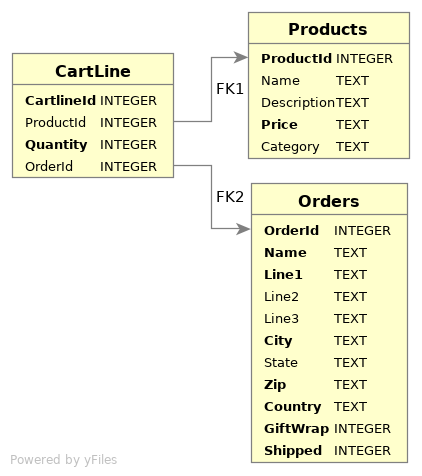
\includegraphics[width=0.7\linewidth]{Images/dbDiagram.png}
 % dbDiagram.png: 422x476 px, 72dpi, 14.89x16.79 cm, bb=0 0 422 476
 \caption{Tabele i relacje bazy Sportstore.db}
 \label{rys:}
\end{figure}
Schemat bazy \textbf{Sportstore.db} został pokazany na Rysunku 1.
Baza \textbf{Identity.db} została utworzona automatycznie przez mechanizm ASP.NET Core Identity, dlatego umieszczanie jej schematu nie ma sensu.
\paragraph{}
Tabele \texttt{Orders} oraz \texttt{Products} nie wymagają wyjaśnień co do przetrzymywanych w nich informacji. Tabela \texttt{CartLine}  przechowuje pojedynczą ``linię zamówienia'' z koszyka zakupów. Jedno zamówienie może zawierać wiele takich linii: Rysunek 2.
\begin{figure}
 \centering
 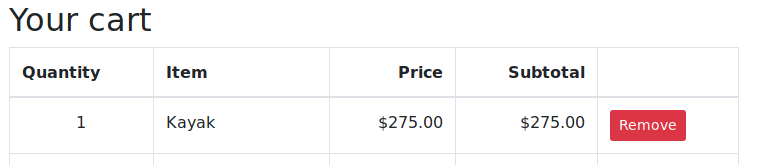
\includegraphics[width=\linewidth]{Images/lineCart.png}
 % lineCart.png: 757x165 px, 72dpi, 26.71x5.82 cm, bb=0 0 757 165
 \caption{Linia zamówienia koszyka zakupów}
 \label{rys:}
\end{figure}


\subsubsection{Autoryzacja użytkownika administracyjnego}
Część administracyjna serwisu jest dostępna tylko po zalogowaniu. Do implementacji wykorzystano ASP.NET Core Identity, ograniczając dostęp do niektórych kontrolerów lub poszczególnych metod za pomocą atrybutu \texttt{[Authorize]}.

\subsubsection{Schemat wyglądu serwisu}
W celu ukształtowania spójnego wyglądu serwisu, wykorzystano poniższe mechanizmy dostępne w ASP.NET Core:
\begin{itemize}
  \item Layouts - współdzielone schematy wyglądu (\texttt{Layout.cshtml} dla części klienckiej oraz \texttt{AdminLayout.cshtml} dla części administracyjnej
 \item ViewComponents - samodzielne komponenty niezależne od kontrolerów (np. \texttt{NavigationMenuViewComponent} odpowiadający za wyświetlanie menu wyboru kategorii).
\end{itemize}
 

\subsubsection{Wyliczenie ilości stron w widoku przeglądania towarów}
Aby prawidłowo wyliczyć liczbę stron pomiędzy którymi możliwa jest nawigacja w przeglądaniu listy towarów, zaimplementowano własny TagHelper. Jest to nowy mechanizm, który pojawił się dopiero w ASP.NET MVC 6 (czyli ASP.NET Core), umożliwiający tworzenie w C\# kodu działającego po stronie HTMLa. Pozwala to na łatwe testowane jednostkowe powstałego kodu oraz jego reużywalność.

\section{Opis działania aplikacji}
\subsection{Część dostępna dla użytkownika}
\subsubsection{Przeglądanie zawartości sklepu}
Przeglądanie zawartości sklepu odbywa się poprzez wybór odpowiedniej kategorii towarów z menu po lewej stronie. W przypadku wybrania \texttt{Home} pokazywane są wszystkie kategorie towarów. Z uwagi na szeroki asortyment sklepu oraz zwiększenie czytelności ograniczono liczbę wyświetlanych towarów do 4. Użytkownik ma możliwość przewijania kolejnych stron listy towarów, jeśli takie istnieją (Rysunek 3).

\begin{figure}
 \centering
 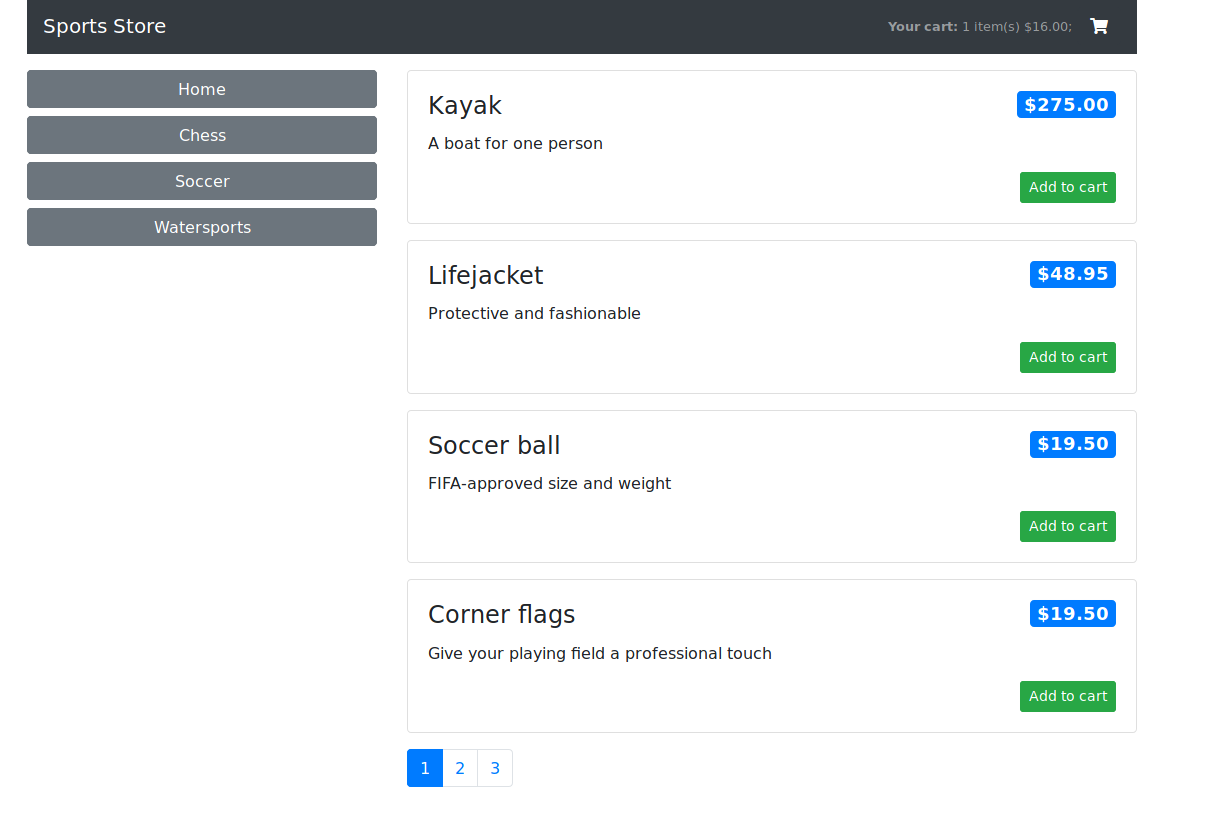
\includegraphics[width=\linewidth]{Images/productsList.png}
 % productsList.png: 1219x821 px, 72dpi, 43.00x28.96 cm, bb=0 0 1219 821
 \caption{Widok przeglądania towarów}
 \label{rys:}
\end{figure}
\subsubsection{Koszyk zakupów}
Po dodaniu towaru do koszyka, wyświetlana jest jego zawartość wraz z możliwością usunięcia towarów. Użytkownik ma możliwość kontynuowania zakupów lub przejścia do widoku złożenia zamówienia (Rysunek 4).

\begin{figure}
 \centering
 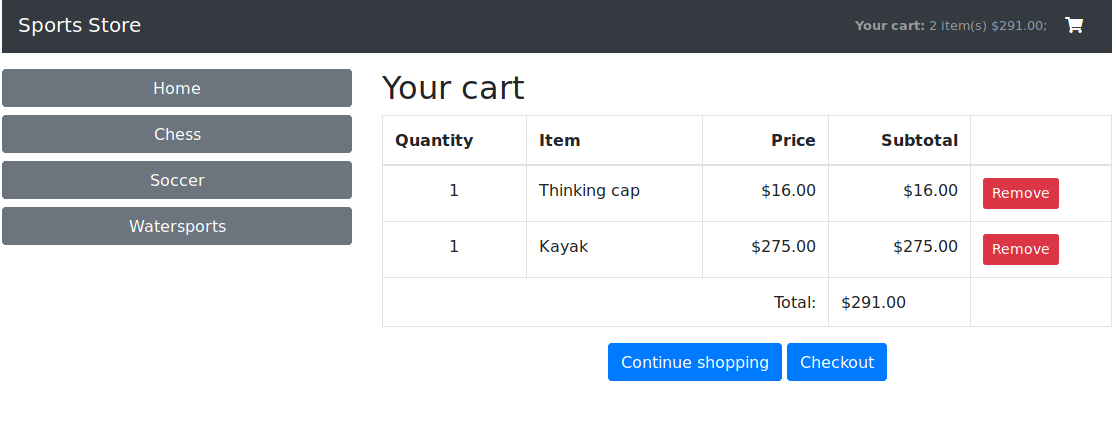
\includegraphics[width=\linewidth]{Images/cart.png}
 % cart.png: 1116x427 px, 72dpi, 39.37x15.06 cm, bb=0 0 1116 427
 \caption{Koszyk zakupów}
 \label{rys:}
\end{figure}
\subsubsection{Złożenie zamówienia}
Składanie zamówienia polega na wypełnieniu danych adresowych oraz opcjonalnych dotyczących pakowania towaru. Formularz jest walidowany po stronie serwera w celu sprawdzenia wypełnienia koniecznych pól (Rysunek 5).
\begin{figure}
 \centering
 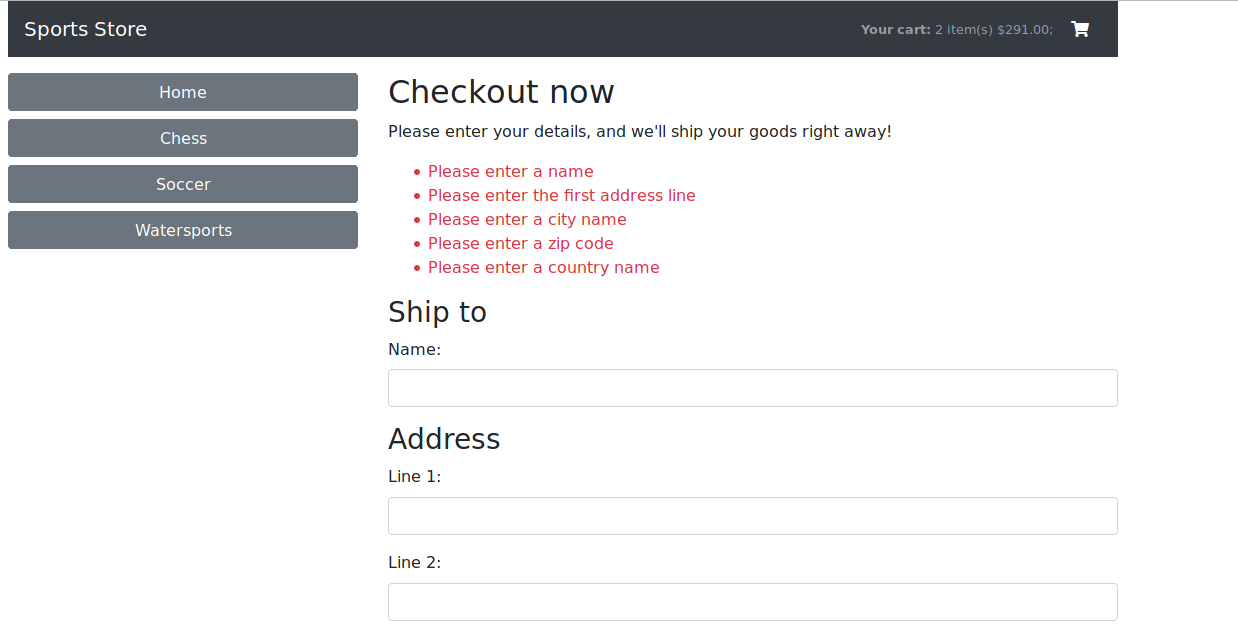
\includegraphics[width=\linewidth]{Images/checkout.png}
 % cart.png: 1116x427 px, 72dpi, 39.37x15.06 cm, bb=0 0 1116 427
 \caption{Widok składania zamówienia (skrócony)}
 \label{rys:}
\end{figure}

\subsection{Część administracyjna}

\end{document}
